\documentclass{beamer} \usetheme{Madrid}
\usecolortheme{beaver}

\usepackage[utf8]{inputenc}
\usepackage{mdframed}
\usepackage{minted}
\usepackage{tikz}
\usepackage{xcolor}
\usetikzlibrary{shapes.geometric, arrows}
\tikzstyle{node} = [rectangle, minimum width=7mm, minimum height=7mm, text centered, fill=gray!30]
\tikzstyle{arrow} = [thick,->,>=stealth]

\definecolor{bg}{rgb}{0.95,0.95,0.95}

\newenvironment{question}[1][]{
	\ifstrempty{#1}{}
	{\mdfsetup{
			frametitle={
					\tikz[baseline=(current bounding box.east),outer sep=0pt]
					\node[anchor=east,rectangle,fill=gray!30]
					{#1};
				}
		}}
	\mdfsetup{
		innertopmargin=10pt,linecolor=gray!30,
		linewidth=2pt,topline=true,
		frametitleaboveskip=\dimexpr - \ht\strutbox\relax
	}
	\begin{mdframed}
		}{
	\end{mdframed}
}

\title{Embedded Systems Programming}
\subtitle{Spring 2021}

\author[]{Jack Leightcap\inst{1}\inst{2}}

% this is pretty pretentious lmao
\institute[IEEE, Wireless Club]{
	\inst{1}IEEE -- \url{nuieeeofficers@gmail.com}
	\and
	\inst{2}Wireless Club -- \url{nuwirelessclub@gmail.com}
}

\date[Spring 2021]{December 6, 2021}

\begin{document}
\frame{\titlepage}

\begin{frame}
	\frametitle{Roadmap}
	\begin{columns}[t]
		\begin{column}{{\textwidth}/2}
			\begin{itemize}
				\item Designed a PCB to connect to Wemos D1 Mini
				\item Soldered it
				\item Now to program with it!
			\end{itemize}
		\end{column}
		\begin{column}{{\textwidth}/2}
			\begin{figure}[H]
				\centering
				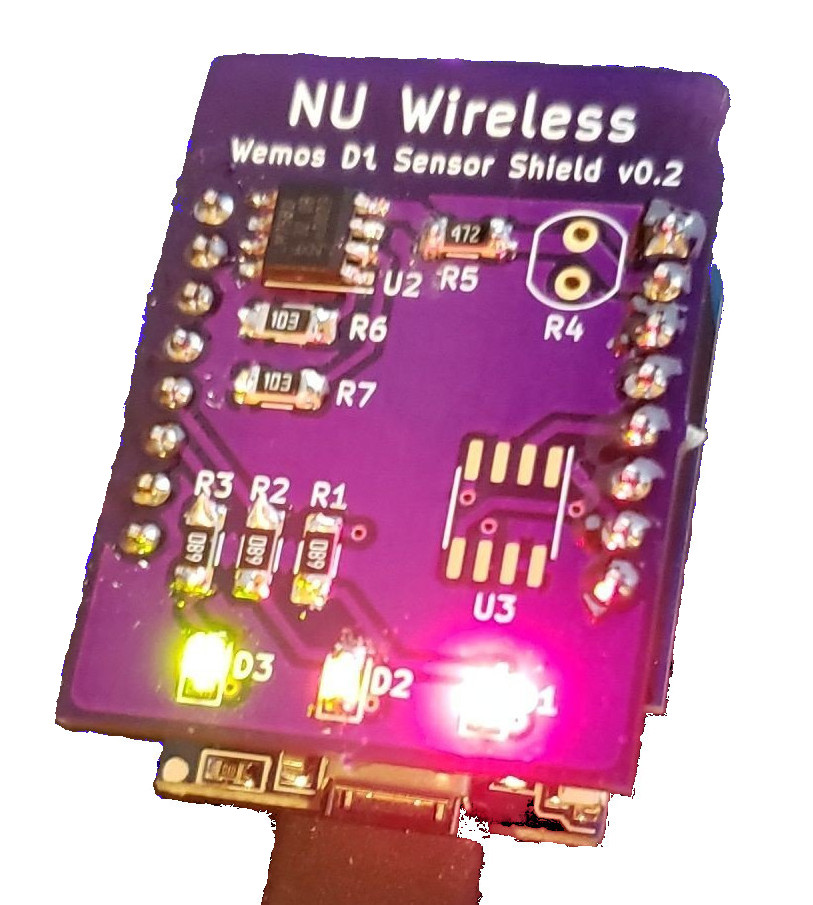
\includegraphics[width=0.7\textwidth]{board.jpeg}
			\end{figure}
		\end{column}
	\end{columns}
\end{frame}

\begin{frame}
	\frametitle{Connecting To Board: Windows}
	\begin{columns}[t]
		\begin{column}{{\textwidth}/2}
			\begin{figure}[H]
				\centering
				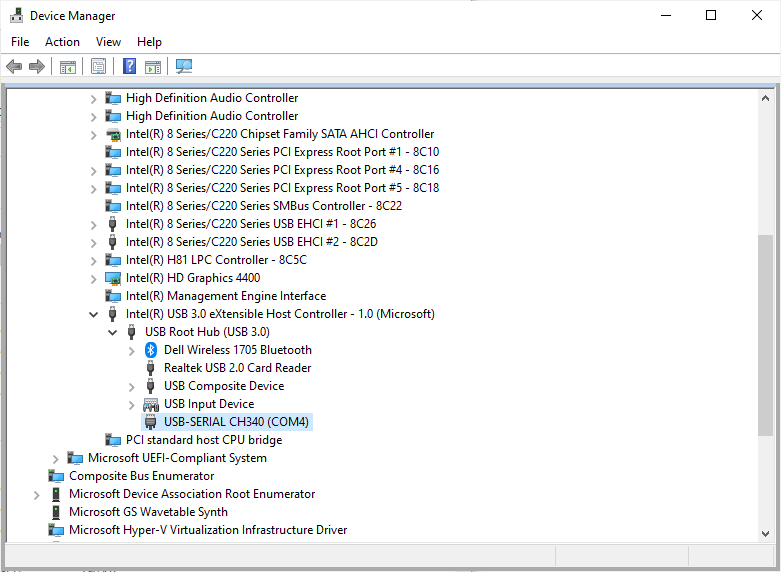
\includegraphics[width=2in]{device.PNG}
				\caption{Find COM Port}
			\end{figure}
		\end{column}
		\begin{column}{{\textwidth}/2}
			\begin{figure}[H]
				\centering
				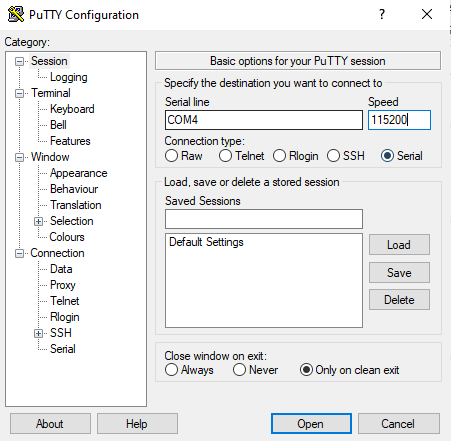
\includegraphics[width=2in]{putty.PNG}
				\caption{Connect with PuTTY}
			\end{figure}
		\end{column}
	\end{columns}
\end{frame}

\begin{frame}[fragile]
	\frametitle{Connecting To Board: MacOS, Linux}
	In a terminal window, use tab completion for exact device:
	\begin{figure}
		\begin{minted}
	[
		frame=lines,
		framesep=2mm,
		fontsize=\small,
		bgcolor=bg
	]
		{bash}
$ screen /dev/ttyUSB* 115200
	\end{minted}
		\caption{Connect with GNU Screen}
	\end{figure}
\end{frame}

\begin{frame}[fragile]
	\frametitle{MicroPython}
	Where are we now?
	\begin{figure}
		\begin{minted}
	[
		frame=lines,
		framesep=2mm,
		fontsize=\footnotesize,
		bgcolor=bg
	]
		{python}
# This '>>>' is a prompt for a Python REPL
>>>
# can do some crazy math
>>> 2 + 2
4
# some more python
>>> list(map(lambda x: chr(x), [72, 105, 33]))
['H', 'i', '!']
# list what files we have around
>>> import os
>>> os.listdir()
['boot.py', 'inet.py', 'led.py', 'light.py', 'main.py', 'temp.py']
	\end{minted}
		\caption{Python REPL}
	\end{figure}
\end{frame}

\begin{frame}[fragile]
	\frametitle{Driver: LEDs}
	\begin{itemize}
		\item Want to be able to control the board's LEDs
		\item The embedded programming equivalent of ``Hello, World!''
	\end{itemize}
	\begin{figure}[H]
		\centering
		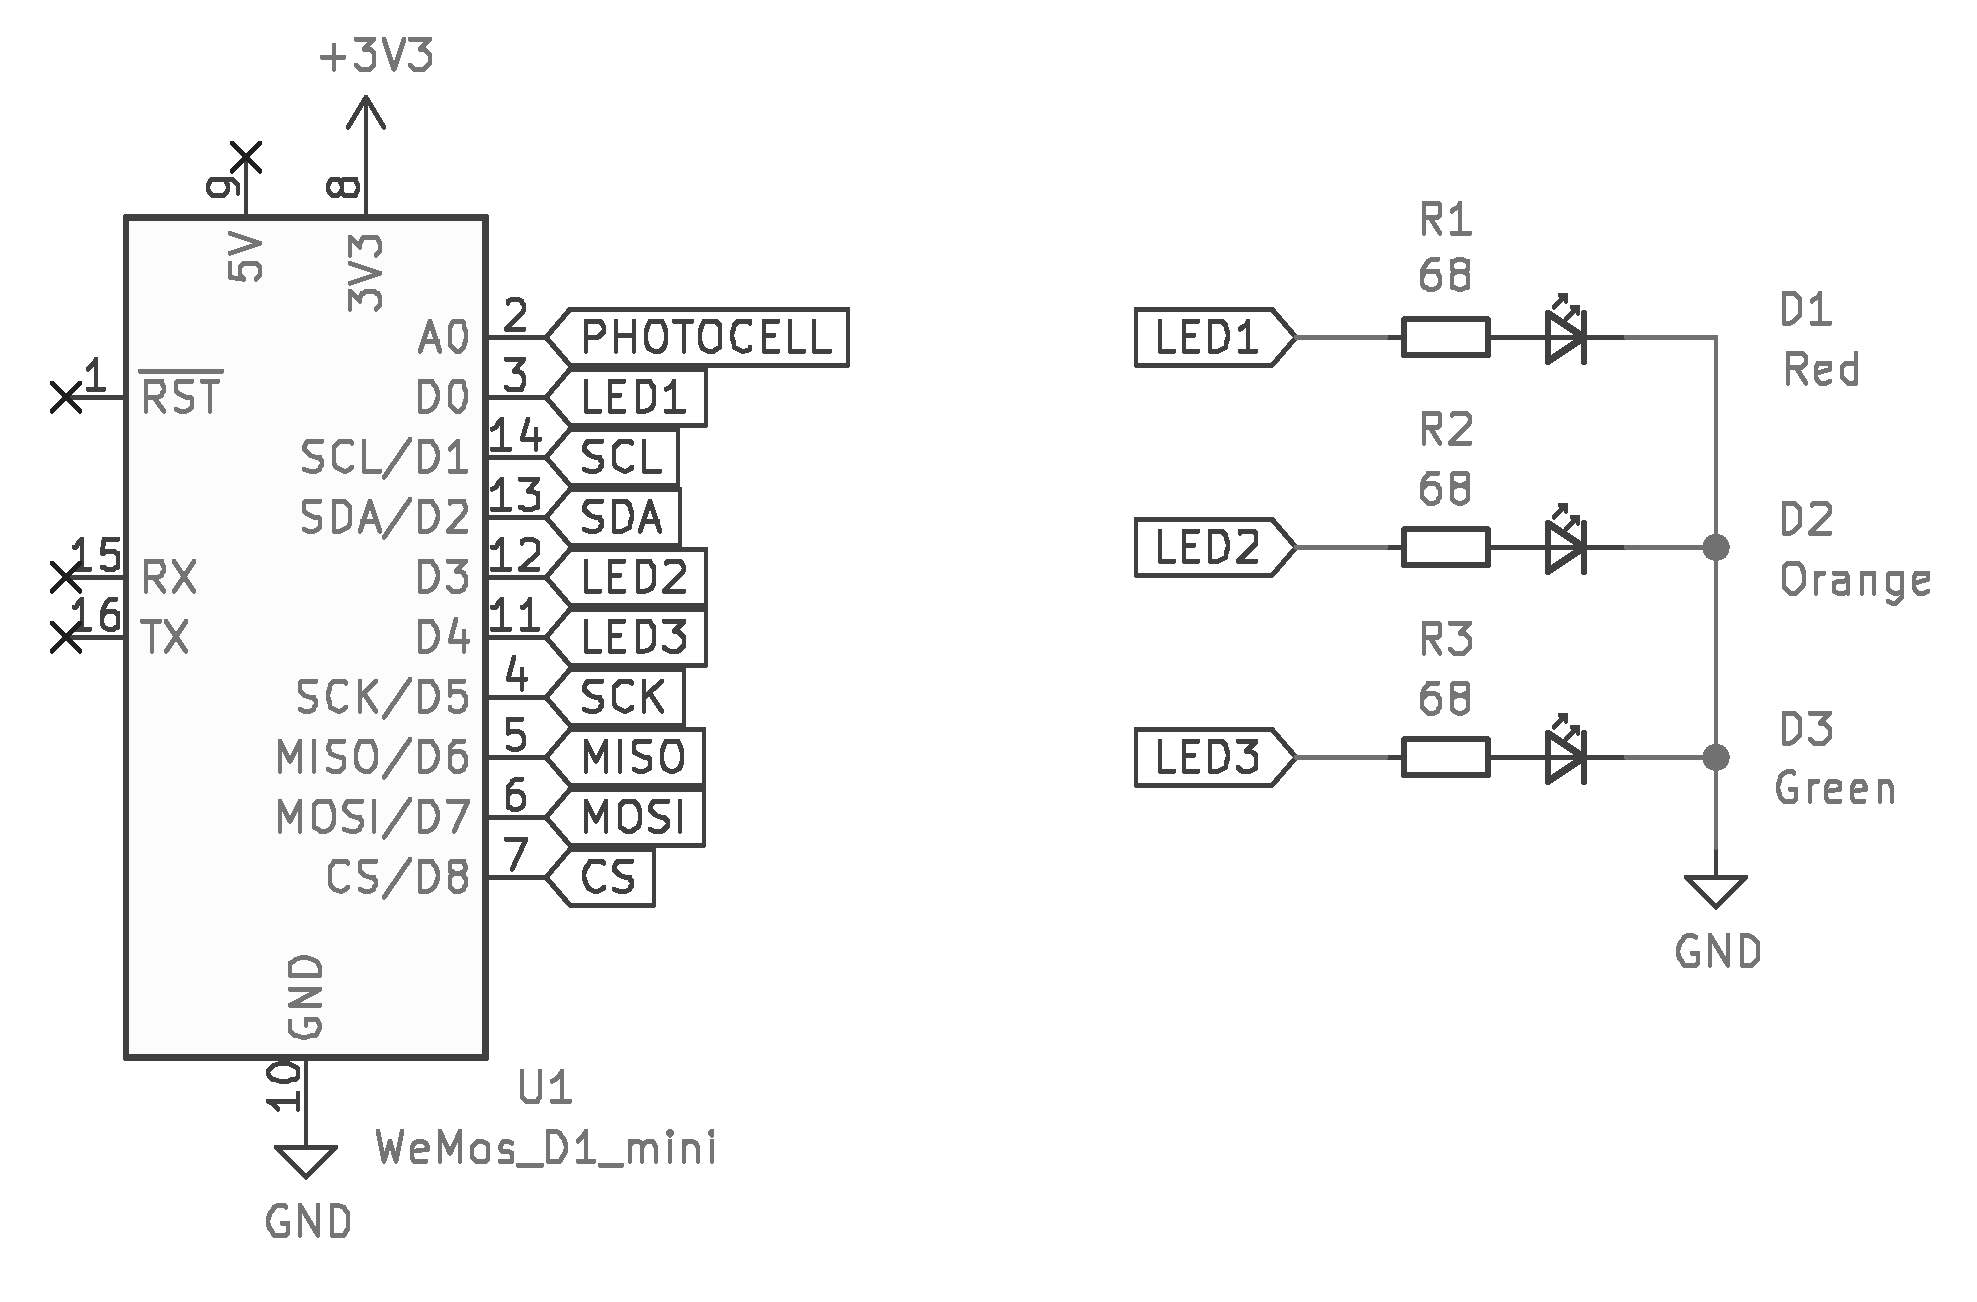
\includegraphics[height=2in]{led_schematic.png}
		\caption{Relevant Schematic Pieces}
	\end{figure}
\end{frame}

\begin{frame}[fragile]
	\frametitle{Driver: LEDs -- First Attempt}
	\begin{minted}
	[
		frame=lines,
		framesep=2mm,
		fontsize=\footnotesize,
		bgcolor=bg
	]
	{python}
>>> import machine
>>> red = machine.Pin(0, machine.Pin.OUT) # D0
>>> orange = machine.Pin(3, machine.Pin.OUT) # D3
>>> green = machine.Pin(4, machine.Pin.OUT) # D4
>>> green.on() # ???
	\end{minted}
\end{frame}

\begin{frame}[fragile]
	\frametitle{Driver: LEDs -- Physical Versus Mapped Pins}
	MicroPython uses \emph{physical pins} of the ESP8266, not the \emph{mapped pins} (\texttt{D0}, etc.) of the Wemos specifically.
	\begin{columns}[t]
		\begin{column}{{\textwidth}/3}
			\begin{figure}[H]
				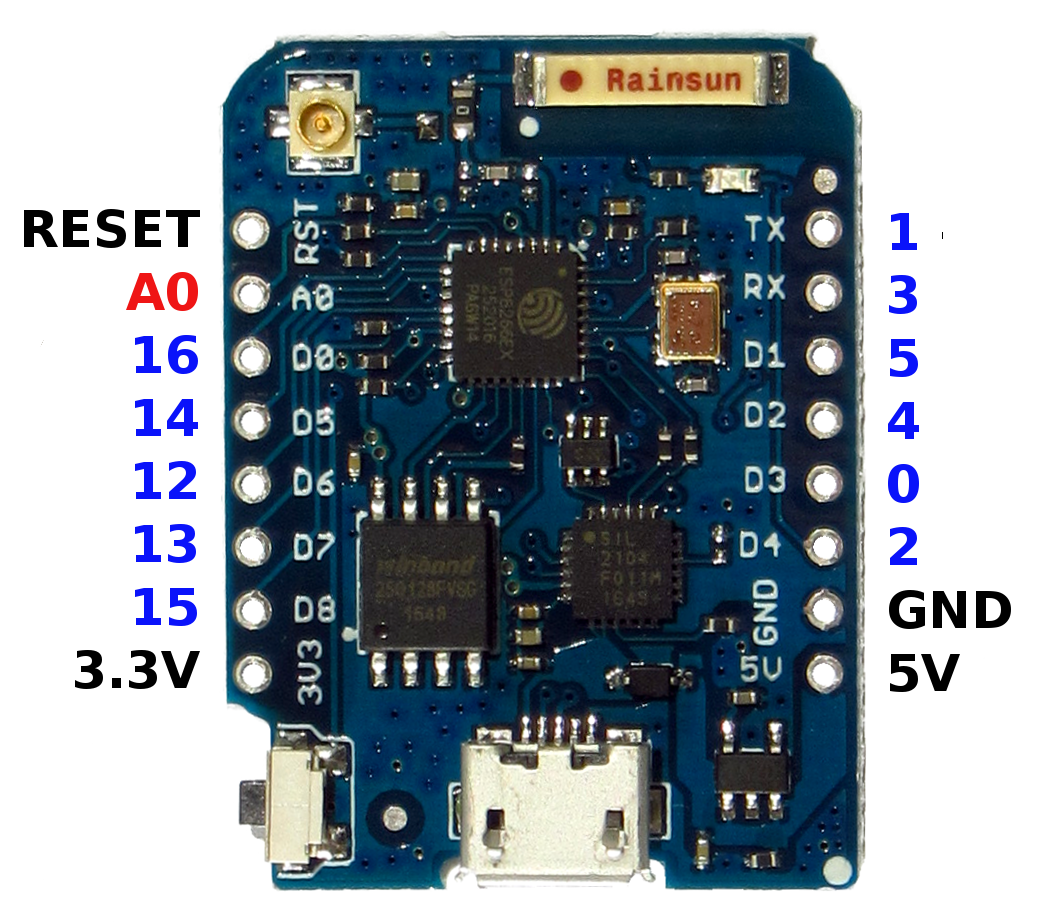
\includegraphics[width=\textwidth]{pinout.png}
				\caption{ESP8266 Pin Map}
			\end{figure}
		\end{column}
		\begin{column}{{2\textwidth}/3}
			\begin{minted}
	[
		frame=lines,
		framesep=2mm,
		fontsize=\footnotesize,
		bgcolor=bg
	]
			{python}
>>> import machine
>>> red = machine.Pin(16, machine.Pin.OUT)
>>> orange = machine.Pin(0, machine.Pin.OUT)
>>> green = machine.Pin(2, machine.Pin.OUT)
>>> green.on() # :^D
>>> green.off()
>>> # encapsulated in a driver:
>>> import led
>>> leds = led.LED()
>>> leds.set("GREEN", False)
	\end{minted}
		\end{column}
	\end{columns}
\end{frame}

\begin{frame}[fragile]
	\frametitle{Driver: LEDs -- Toggling}
	\begin{minted}
	[
		frame=lines,
		framesep=2mm,
		fontsize=\footnotesize,
		bgcolor=bg
	]{python}
>>> import machine
>>> import time
>>> while True:
...     red.on() if red.value() == 0 else red.off()
...     time.sleep(1)

	\end{minted}
	what happens now? (\texttt{CTRL+C} stops)
\end{frame}

\begin{frame}[fragile]
	\frametitle{Driver: LEDs -- Toggling, Timers}
	\begin{minted}
	[
		frame=lines,
		framesep=2mm,
		fontsize=\footnotesize,
		bgcolor=bg
	]{python}
>>> from machine import Timer
>>> timer = Timer(-1)
# the callback is provided one argument -- we ignore it
>>> f = lambda _: red.on() if red.value() == 0 else red.off()
# start a periodic timer with period 1000ms
>>> timer.init(period=1000, mode=Timer.PERIODIC, callback=f)
	\end{minted}
	why does this work?
\end{frame}

\begin{frame}[fragile]
	\frametitle{Driver: Light Sensor}
	\emph{ADC} -- Analog-Digital Converter
	\begin{columns}[t]
		\begin{column}{{\textwidth}/3}
			\begin{figure}[H]
				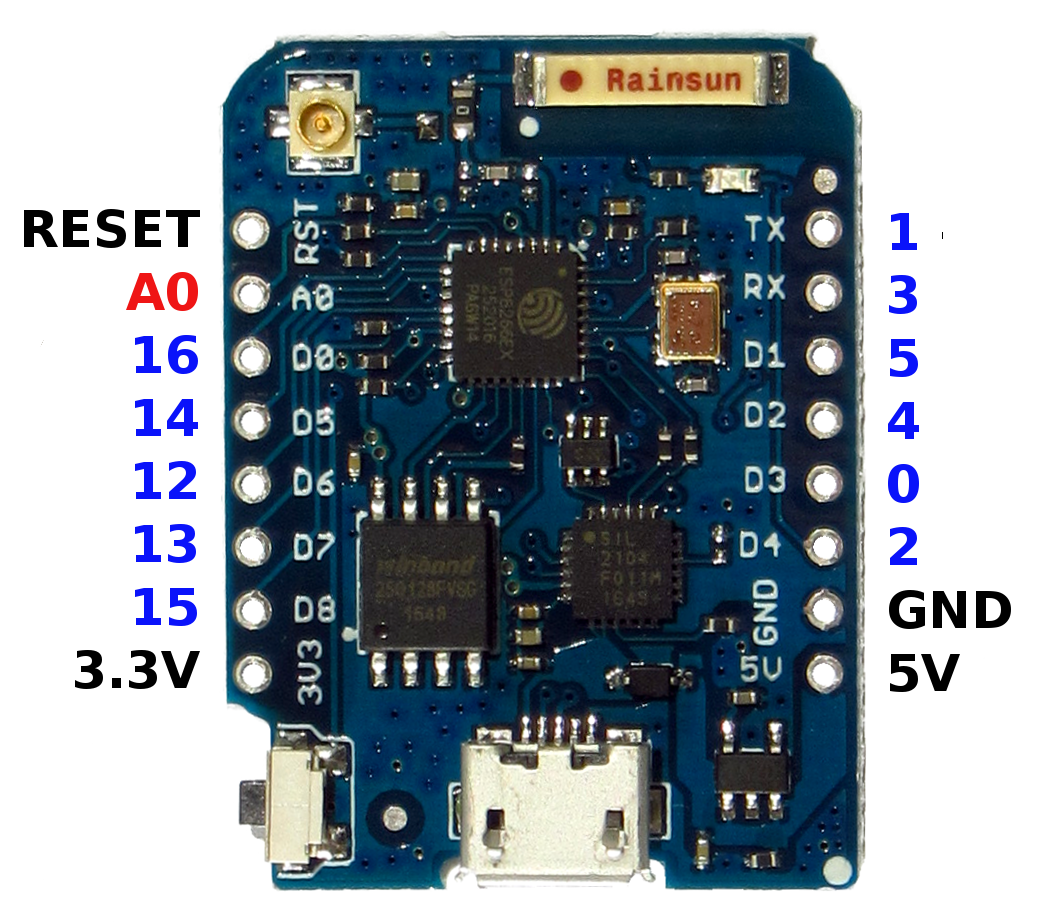
\includegraphics[width=\textwidth]{pinout.png}
				\caption{ESP8266 Pin Map}
			\end{figure}
		\end{column}
		\begin{column}{{2\textwidth}/3}
			\begin{minted}
	[
		frame=lines,
		framesep=2mm,
		fontsize=\footnotesize,
		bgcolor=bg
	]
			{python}
>>> import machine
>>> light = machine.ADC(0)
>>> light.read()
123
>>> light.read() # put finger over photocell
34
>>> # encapsulated in a driver:
>>> import light
>>> lightsensor = light.LightSensor()
>>> lightsensor.read()
...
	\end{minted}
		\end{column}
	\end{columns}
\end{frame}

\begin{frame}[fragile]
	\frametitle{Driver: Temperature Sensor}
	\begin{itemize}
		\item Uses \texttt{I2C} (\emph{Inter-Integrated Circuit})
		      \begin{itemize}
			      \item \emph{Serial} -- Send one bit at a time over one wire, spread over time
			      \item \emph{Parallel} -- Send multiple bits at a time at once, over multiple wires
		      \end{itemize}
		\item Read a lots of documentation to get bespoke numbers...
	\end{itemize}
	\begin{minted}
	[
		frame=lines,
		framesep=2mm,
		fontsize=\footnotesize,
		bgcolor=bg
	]
			{python}
>>> import machine
>>> i2c = machine.I2C(freq=400000, # frequency
                      scl=machine.Pin(5, machine.Pin.OUT), # clock
                      sda=machine.Pin(4)) # data
>>> i2c.writeto(72, b'00000000')
>>> output = i2c.readfrom(72, 2)
>>> output = int.from_bytes(output, "big")
>>> (output >> 5) / 8
32.5
>>> # encapsulated in a driver:
>>> import temp
>>> tempsensor = temp.TempSensor()
>>> tempsensor.read() # turns out this sensor isn't very accurate
32.5
	\end{minted}
\end{frame}

\begin{frame}[fragile]
	\frametitle{Driver: Internet}
	\begin{columns}[t]
		\begin{column}{{2\textwidth}/3}
			\begin{itemize}
				\item Put it all together!
				\item (Not that exciting to implement...)
			\end{itemize}
			\begin{minted}
	[
		frame=lines,
		framesep=2mm,
	fontsize=\footnotesize,
	bgcolor=bg
	]
			{python}
>>> import inet
>>> internet = inet.WebDriver("SSID", "pword")
Connection successful
('192.168.4.1', '255.255.255.0', ...)
>>> internet.serve(
  ["The temperature is:",
   "The light is:"],
  [tempsensor.read,
   lightsensor.read]
)
# connect your phone to that SSID...
# go to that IP address...
	\end{minted}
		\end{column}
		\begin{column}{{\textwidth}/3}
			\begin{figure}[H]
				\centering
				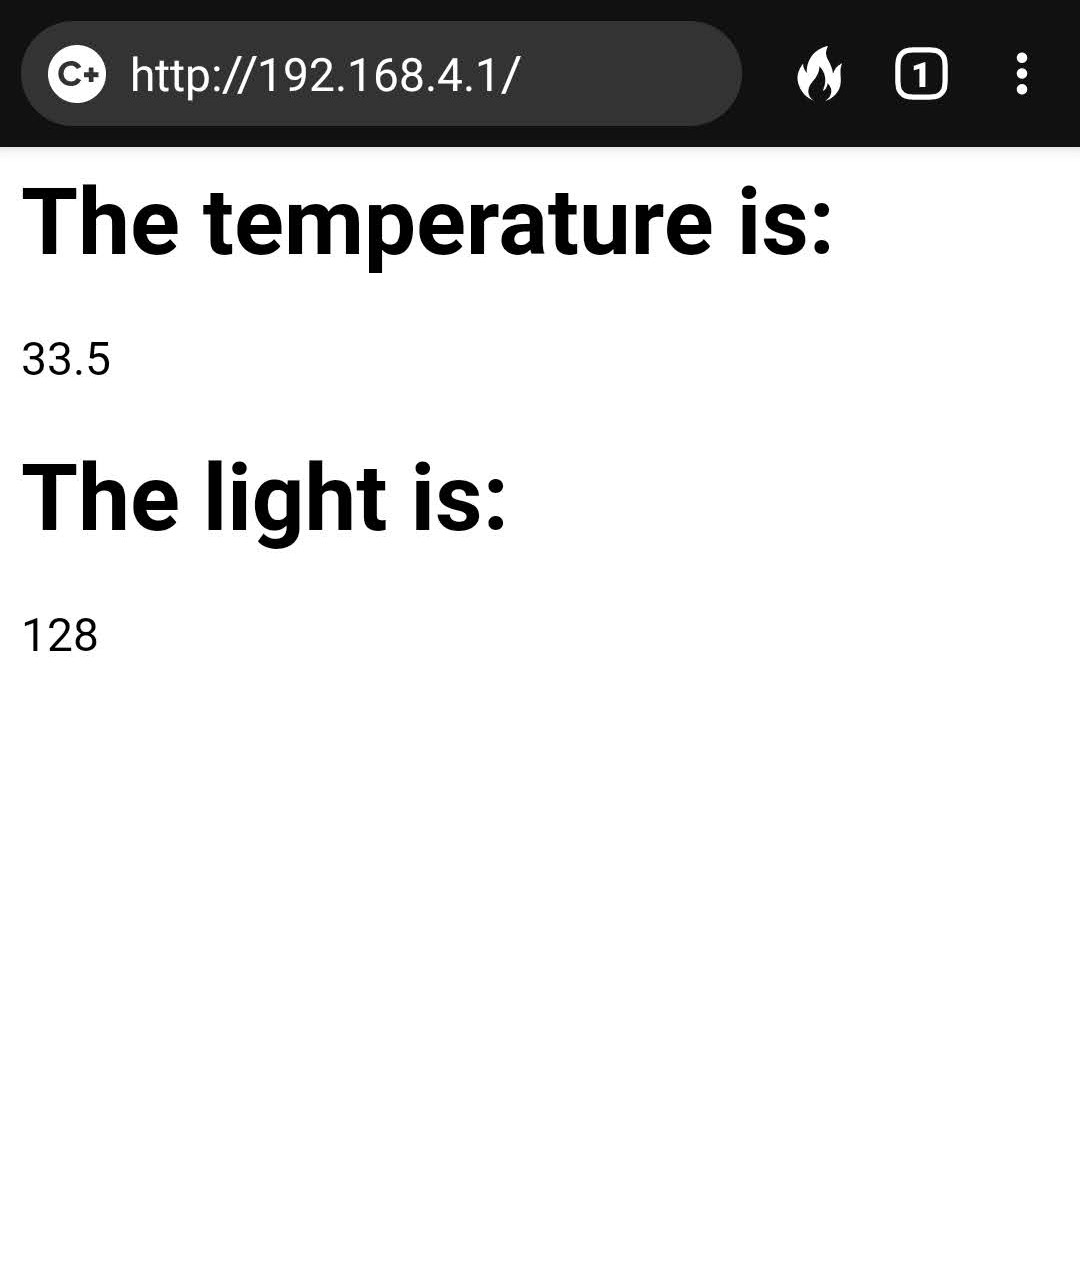
\includegraphics[width=\textwidth]{inet.jpg}
				\caption{Readings on Phone}
			\end{figure}
		\end{column}
	\end{columns}
\end{frame}

\begin{frame}
	\frametitle{Resources}
	\begin{itemize}
		\item Drivers: \url{https://github.com/jleightcap/wemos-sensors-upython}
		\item ESP8266 Firmware with built-in drivers: \url{https://github.com/jleightcap/micropython}
		\item Slides:
		      \url{https://raw.githubusercontent.com/NEUWireless/Workshops/master/embedded-spring2021/slides.pdf}
	\end{itemize}
\end{frame}

\end{document}
